\documentclass[10pt]{article}
\usepackage{float}
\usepackage[utf8]{inputenc}
\usepackage[OT1]{fontenc}
\usepackage{amsfonts, amsmath, amsthm, amssymb}
\usepackage{bbm}
\usepackage{mathtools}
\usepackage{natbib}
\usepackage{graphicx}
\usepackage{listings}
\usepackage[margin=1in]{geometry}
\usepackage{xcolor}
\usepackage{bigints}
\usepackage{glossaries}
\usepackage{graphicx}
\usepackage{enumerate}

\theoremstyle{definition}
\newtheorem{definition}{Definition}[section]

\newtheorem{theorem}{Theorem}
\newtheorem{proposition}{Proposition}
\newtheorem{example}{Example}

\newcounter{countCode}
\lstnewenvironment{code} [1][caption=Ponme caption, label=default]{%
	\renewcommand*{\lstlistingname}{Listado} 
	\setcounter{lstlisting}{\value{countCode}} 
	\lstset{ %
	language=java,
	basicstyle=\ttfamily\footnotesize,       % the size of the fonts that are used for the code
	numbers=left,                   % where to put the line-numbers
	numberstyle=\sc,      % the size of the fonts that are used for the line-numbers
	stepnumber=1,                   % the step between two line-numbers. 
	numbersep=5pt,                 % how far the line-numbers are from the code
	numberstyle=\color{red!50!blue},
    	backgroundcolor=\color{lightgray!20},
	rulecolor=\color{blue},
	keywordstyle=\color{red}\bfseries,
	showspaces=false,               % show spaces adding particular underscores
	showstringspaces=false,         % underline spaces within strings
	showtabs=false,                 % show tabs within strings adding particular underscores
	frame=single,                   % adds a frame around the code
	framexleftmargin=0mm,
	numberblanklines=false,
	xleftmargin=5pt,
	breaklines=true,
	breakatwhitespace=true,
	breakautoindent=true,
	captionpos=t,
	texcl=true,
	tabsize=2,                      % sets default tabsize to 3 spaces
	extendedchars=true,
	inputencoding=utf8, 
	escapechar=\%,
	morekeywords={print, println, size, background, strokeWeight, fill, line, rect, ellipse, triangle, arc, save, PI, HALF_PI, QUARTER_PI, TAU, TWO_PI, width, height,},
	emph=[1]{print,println,}, emphstyle=[1]{\color{blue}}, % Mis palabras clave.
	emph=[2]{width,height,}, emphstyle=[2]{\bf\color{violet}}, % Mis palabras clave.
	emph=[3]{PI, HALF_PI, QUARTER_PI, TAU, TWO_PI}, emphstyle=[3]\color{orange!50!violet}, % Mis palabras clave.
	emph=[4]{line, rect, ellipse, triangle, arc,}, emphstyle=[4]\color{green!70!black}, % Mis palabras clave.
	%emph=[5]{size, background, strokeWeight, fill,}, emphstyle=[5]{\tt \color{red!30!blue}}, % Mis palabras clave.
	%emph={[2]sqrt,baset}, emphstyle={[2]\color{blue}}, % f(sqrt(2)), sqrt a nivel 2 se pondrá azul
	#1}}{\addtocounter{countCode}{1}}



\title{Dataset Transferability Analysis via Optimal Transport}
\author{Davi Sales Barreira}
\date{\today}
\begin{document}
\maketitle

\section{Introduction}

Optimal Transport (OT) theory is a field of mathematics that studies the problem of optimally transporting
quantities from one configuration to another given a cost function.
The origin of the field is commonly attributed to the french mathematicians Gaspard Monge (1746-1818)
whose original motivating problem was
``what is the optimal way to transport soil extracted
from one location and move to another where it will be used,
for example, on a construction?'' (see Figure \ref{fig:mongeproblem}).

\begin{figure}[H]
  \centering
  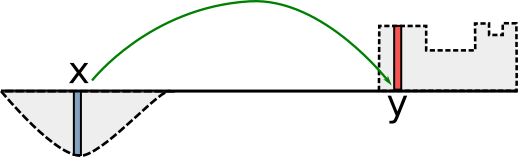
\includegraphics[width=8cm]{Figures/mongeproblem.png}
  \caption{Illustration of the original Monge Problem, where all the mass is excavated from location
  $x$ is transported to a deterministic location $y$. The transport assignment map is represented by the arrow in green.}
  \label{fig:mongeproblem}
\end{figure}

This seemingly narrow subject has actually many applications beyond what one may see at first.
In the field of Machine Learning, Optimal Transport theory has been gaining attention, specially
in subareas such as transfer learning
(\citep{flamary2014optimal}, \citep{courty2014domain},
\citep{damodaran2018deepjdot}, \citep{solomon2014wasserstein},
\citep{shen2018wasserstein}).
One of the main ways in which OT is used in Machine Learning is in order to define
a distance metrics between probability distributions. Note that
two datasets may be interpreted as empirical distributions
in high-dimensions, and one can use Optimal Transport in order to obtain the minimal cost
of transporting one dataset distribution into the other. This cost can be thought of
as a distance measure between datasets.

This project is based on the work of \citet{alvarez2020geometric}, where the
authors proposed one way of measuring the distance between datasets using
Optimal Transport. Their metric, which was called Optimal Transport
Dataset Distance (OTDD), was shown to be correlated to performance in terms of
transfer learning, i.e. the lower the OTDD, the better was the transfer learning
between two datasets. Hence, the OTDD could be
used as a parameter to evaluate how well the transfer learning would be
between two datasets.

Suppose that you have many
datasets which you can train to then use a transfer learning method
in order to make prediction in another dataset. Hence,
\citet{alvarez2020geometric} proposed the use of OTDD as a metric
in order to evaluate which dataset would be best suited.

In this project, we make use of the OTDD metric to evaluate
the transferability between two datasets, but instead of
comparing many datasets, we develop a tool that allows users
to explore the differences between the datasets, and perform data
augmentations in order to improve the transferability between the datasets, i.e.
reduce the OTDD distance.


% \nocite{*}

  \bibliography{ref}
  \bibliographystyle{plainnat}
\end{document}

